\documentclass[tikz,border=2pt]{standalone}
\usepackage{amsmath}
\usepackage{pgfplots}
\pgfplotsset{compat=1.18}
\usetikzlibrary{arrows.meta}
\begin{document}
% Job market, w(1) = 2, w(0) = 1 in the candidate separating profile (H educates, L does not).
% Incentive constraints: H: c_H <= 1, L: c_L >= 1. The shaded set is where the separating PBE
% exists; (0.5, 1.5) is inside, (0.5, 0.8) is outside because L would mimic (2 - 0.8 = 1.2 > 1).
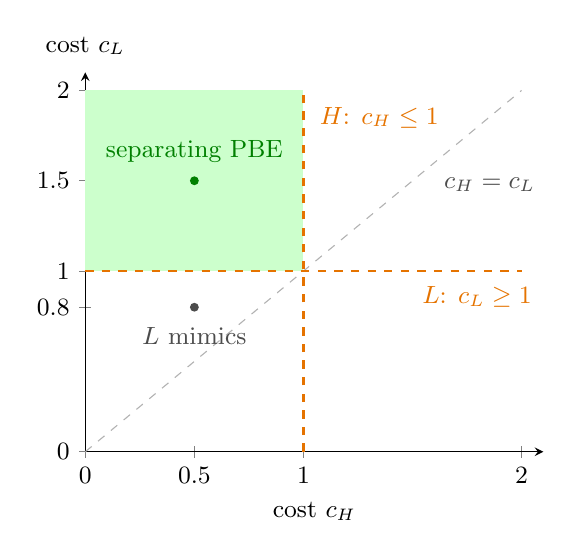
\begin{tikzpicture}[font=\small, >={Latex[length=2mm]}]
  \begin{axis}[
    axis lines=left, xmin=0, xmax=2.1, ymin=0, ymax=2.1,
    xtick={0,0.5,1,2}, ytick={0,0.8,1,1.5,2},
    xticklabels={$0$,$0.5$,$1$,$2$}, yticklabels={$0$,$0.8$,$1$,$1.5$,$2$},
    xlabel={cost $c_H$}, ylabel={cost $c_L$},
    ylabel style={rotate=-90, anchor=south, at={(axis description cs:0,1.02)}},
    width=7.4cm, height=6.4cm, clip=false]
    \addplot[fill=green!20, draw=none] coordinates {(0,1) (1,1) (1,2) (0,2)} -- cycle;
    \addplot[gray!60, thin, dashed] coordinates {(0,0) (2,2)};
    \addplot[orange!90!black, thick, dashed] coordinates {(1,0) (1,2)};
    \addplot[orange!90!black, thick, dashed] coordinates {(0,1) (2,1)};
    \fill[green!50!black] (axis cs:0.5,1.5) circle (1.6pt);
    \fill[gray!60!black] (axis cs:0.5,0.8) circle (1.6pt);
    \node[green!50!black, anchor=south] at (axis cs:0.5,1.55) {separating PBE};
    \node[gray!60!black, anchor=north] at (axis cs:0.5,0.74) {$L$ mimics};
    \node[orange!90!black, anchor=west] at (axis cs:1.03,1.85) {$H$: $c_H\le1$};
    \node[orange!90!black, anchor=north west] at (axis cs:1.5,0.97) {$L$: $c_L\ge1$};
    \node[gray!60!black, anchor=west] at (axis cs:1.6,1.48) {$c_H=c_L$};
  \end{axis}
\end{tikzpicture}
\end{document}
